\documentclass{article}
\usepackage{amsmath}
\usepackage{tikz}
\usetikzlibrary{arrows.meta}

\begin{document}

\begin{center}
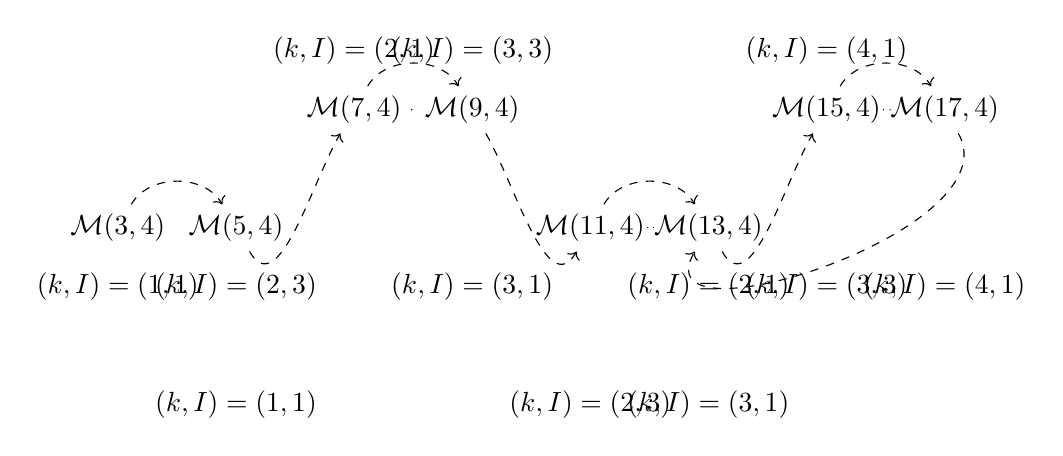
\begin{tikzpicture}[scale=1.5]
    % Nodes representing the modular categories
    \node (M34) at (-2,0) {$\mathcal{M}(3,4)$};
    \node (M54) at (-1,0) {$\mathcal{M}(5,4)$};
    \node (M74) at (0,1) {$\mathcal{M}(7,4)$};
    \node (M94) at (1,1) {$\mathcal{M}(9,4)$};
    \node (M114) at (2,0) {$\mathcal{M}(11,4)$};
    \node (M134) at (3,0) {$\mathcal{M}(13,4)$};
    \node (M154) at (4,1) {$\mathcal{M}(15,4)$};
    \node (M174) at (5,1) {$\mathcal{M}(17,4)$};

    % Nodes representing the (k,I) pairs
    \node (k11) at (-2,-0.5) {$(k,I)=(1,1)$};
    \node (k23) at (-1,-0.5) {$(k,I)=(2,3)$};
    \node (k31) at (1,-0.5) {$(k,I)=(3,1)$};
    \node (k21) at (3,-0.5) {$(k,I)=(2,1)$};
    \node (k33) at (4,-0.5) {$(k,I)=(3,3)$};
    \node (k41) at (5,-0.5) {$(k,I)=(4,1)$};

    % Arrows connecting the nodes
    \draw[->,dashed] (M34) to [out=60,in=120] (M54);
    \draw[->,dashed] (M54) to [out=-60,in=-120] (M74);
    \draw[->,dashed] (M74) to [out=60,in=120] (M94);
    \draw[->,dashed] (M94) to [out=-60,in=-120] (M114);
    \draw[->,dashed] (M114) to [out=60,in=120] (M134);
    \draw[->,dashed] (M134) to [out=-60,in=-120] (M154);
    \draw[->,dashed] (M154) to [out=60,in=120] (M174);
    \draw[->,dashed] (M174) to [out=-60,in=-120] (M134);

    % Dotted arrows indicating possible flows
    \draw[dotted] (M74) -- (M94);
    \draw[dotted] (M114) -- (M134);
    \draw[dotted] (M154) -- (M174);

    % Labels for the (k,I) pairs
    \node at (0,1.5) {$(k,I)=(2,1)$};
    \node at (1,1.5) {$(k,I)=(3,3)$};
    \node at (4,1.5) {$(k,I)=(4,1)$};
    \node at (2,-1.5) {$(k,I)=(2,3)$};
    \node at (3,-1.5) {$(k,I)=(3,1)$};
    \node at (-1,-1.5) {$(k,I)=(1,1)$};
\end{tikzpicture}
\end{center}

\textbf{\caption{$\mathcal{M}(p,4)$ are classified in terms of the spin contents and the quantum dimensions of the duality defect $\mathcal{N}$. They constrain the renormalization group flow like this figure. Dotted arrows are possible in the half-integer $k$ flow which does not preserve the duality defect lines.}}
\end{document}